\documentclass[10pt]{article}
\usepackage{graphicx}
\usepackage{amssymb}
\usepackage[fleqn]{amsmath}
\usepackage{nccmath}
\usepackage{cases}
\usepackage{hyperref}
\usepackage{pgfplots}
\usepackage{enumitem}
\pgfplotsset{compat=1.18}
\usepackage{float}
\usepackage{pdfpages}
\DeclareMathOperator*{\argmax}{argmax\,}
\DeclareMathOperator*{\argmin}{argmin\,}

\title{\bf Math 156: Problem Set 3}
\author{\bf Owen Jones}
\begin{document}
\section*{Problem 1}
\begin{itemize}
    \item [(a)] Assume to the contrary we have some $\mathbf{w},b,\xi$ that minimizes the objective function under the given constraints s.t $\exists\xi_k(\xi_k<0)$.
    Define a new $\xi'_n:=\max(0,\xi_n)$. 
    Because $\xi_k^2>{\xi_k'}^2$, it follows\\ 
    $\displaystyle \frac{1}{2}{\lVert \mathbf{w}\rVert}^2_2+C\xi_k^2+C\sum_{n=1\atop n\neq k}^{N}\xi_n^2>\frac{1}{2}{\lVert \mathbf{w}\rVert}^2_2+C\sum_{n=1}^{N}{\xi_n'}^2$.\\
    It suffices to show $\xi'$ satisfies $t_n(\mathbf{w}^\top\phi(x_n)+b)\ge 1-\xi_n'$.\\
    $t_n(\mathbf{w}^\top\phi(x_n)+b)\ge 1-\xi_n\ge 1-\xi_n'$ because $\xi_n'\ge\xi_n(\forall n)$, so $\xi'$ also satisfies the given constraints.
    Hence, we obtain a contradiction because any solution containing $\xi_k<0$ can't be a minimizer, so the $\xi_n\ge0\quad\forall n$ doesn't affect the optimal solution.
    \item [(b)] $C$ is a regularization parameter that controls the tradeoff between maximizing the margin and maximizing the classification error.
    Increasing $C$ leads to a smaller margin, but fewer misclassifications on the training set. This can lead to greater variance and overfitting.
\end{itemize}
\section*{Problem 2}
Assume we have some $\mathbf{w}_0$ and $b_0$ s.t all points satisfy the constraint in Eq (7.5) and maximizes Eq (7.3). 
It follows the hyperplane $\mathbf{w}_0^\top x+b_0=0$ is the optimal classification margin. 
Suppose the constraint in Eq (7.5) becomes 
\begin{equation*}
t_n(\mathbf{w}^\top\mathbf{\phi}(x_n)+b)\ge \gamma\quad\forall n
\end{equation*}  
If we perform the change of variables $\mathbf{w}_0\rightarrow \gamma \mathbf{w}_0$ and $b_0\rightarrow \gamma b_0$, the new constraint will be satisfied and Eq (7.3) will still be maximized.
The new hyperplane $\gamma\mathbf{w}_0^\top x+\gamma b_0=0$ is the optimal classification margin. 
However, the new hyperplane is equivalent to the old hyperplane ($\gamma\mathbf{w}_0^\top x+\gamma b_0=0$ iff $\mathbf{w}_0^\top x+b_0=0$).
Moreover, the minimum distance to the hyperplane remains the same ($\frac{t_n (\gamma\mathbf{w}^\top \phi(x_n)+\gamma b)}{\lVert\gamma\mathbf{w}\rVert}=\frac{\gamma t_n (\mathbf{w}^\top \phi(x_n)+b)}{\gamma\lVert\mathbf{w}\rVert}=\frac{t_n (\mathbf{w}^\top \phi(x_n)+b)}{\lVert\mathbf{w}\rVert}$).
\section*{Problem 3}
% Preprocessing:\\
% Applied scikit-learn's Standard Scaler to standardize the features. 
% Split the dataset into training and test sets. 
% Fit scikit-learn's PCA to the training data and performed the transformation on the training and test sets. 
% Set to preserve $95\%$ of explained variance.\\
% K-Nearest Neighbors:\\
% Tested number of nearest neighbors: $[5,10,15,20]$\\
% Used scikit-learn's GridSearchCV with $3$ folds to train model\\
% Best parameter: $5$ neighbors\\
Preprocessing: The steps I took to preprocess the MNIST dataset were as follows: applied scikit-learn's Standard Scaler to the entire dataset, split into training $(80\%)$ and test $(20\%)$, fit a PCA to the training set that preserved $95\%$ of the explained variance, applied PCA transformation to the train and test set.\\ 
K-Nearest Neighbors tested number of nearest neighbors $[5,10,15,20]$. Used scikit-learn's GridSearchCV with $3$ folds to train model. $5$ neighbors performed the best.\\
Across the board model performed very well on the test set. Performed best overall. Class-$8$ only had a $91\%$ recall most often misclassifying $8$s as $5$s (falsely classified as $5$s). Otherwise, all metrics in the mid to high $90\%$.\\
Accuracy: $95\%$, Precision: $95\%$, Recall: $95\%$, f-1 score: $95\%$\\
Logistic Regression tested the regularization value $C$ (inverse of regularization strength) $[0.001,0.01,0.1,1,10,100]$. Used scikit-learn's GridSearchCV with $3$ folds to train model. $C=1$ performed the best.\\
Model performed pretty well on the test set. Model did not perform as well classifying $3s,5s,8s$, and $9s$. $3,5$, and $8$ had slightly lower recalls than the other classes, and $8$ and $9$ had slightly lower precisions.\\
Accuracy: $92\%$, Precision: $92\%$, Recall: $92\%$, f-1 score: $92\%$\\
Decision tree tested max depth of the tree $[None, 5, 10, 15, 20]$. Used scikit-learn's GridSearchCV with $5$ folds to train model. max depth=$15$ performed the best.\\
Model performed the worst relative to other models. Did not perform well classifying $3s,5s,8s$, and $9s$ as with Logistic Regression. $3,5,8$, and $9$ had lower recalls whereas $5,8$, and $9$ had lower precisions.\\
Accuracy: $83\%$, Precision: $83\%$, Recall: $83\%$, f-1 score: $83\%$\\
Linear svm classification tested the regularization value $C$ $[0.001,0.01,0.1,1]$. Used scikit-learn's GridSearchCV with $2$ folds to train model. $C=0.01$ performed the best.\\
Note: $C=0.001$ took about $~10\%$ the time it took to fit as the other tested values, and the accuracies were all within less than $0.5\%$.
Like previous models, performs slightly worse on $3s,5s,8s$, and $9s$ (both accuracy and precision).\\
Accuracy: $91\%$, Precision: $91\%$, Recall: $91\%$, f-1 score: $91\%$\\
Svm classification tested the different kernels linear,poly,rbf, and sigmoid. Used scikit-learn's GridSearchCV with $5$ folds to train model and $C=0.001$. The linear kernel performed the best.\\
Other kernels don't perform nearly as well. Linear kernel performs pretty well across the board. Slightly worse recall on $5s$.\\
Used $C=0.001$ instead of $C=0.01$ to reduce training time. Tested the hyperparameters $C$, kernel individually to reduce training time as well.\\
Accuracy: $94\%$, Precision: $94\%$, Recall: $94\%$, f-1 score: $94\%$\\
K-Nearest Neighbors performed the best in comparison to other models and didn't take very long to fit/score.
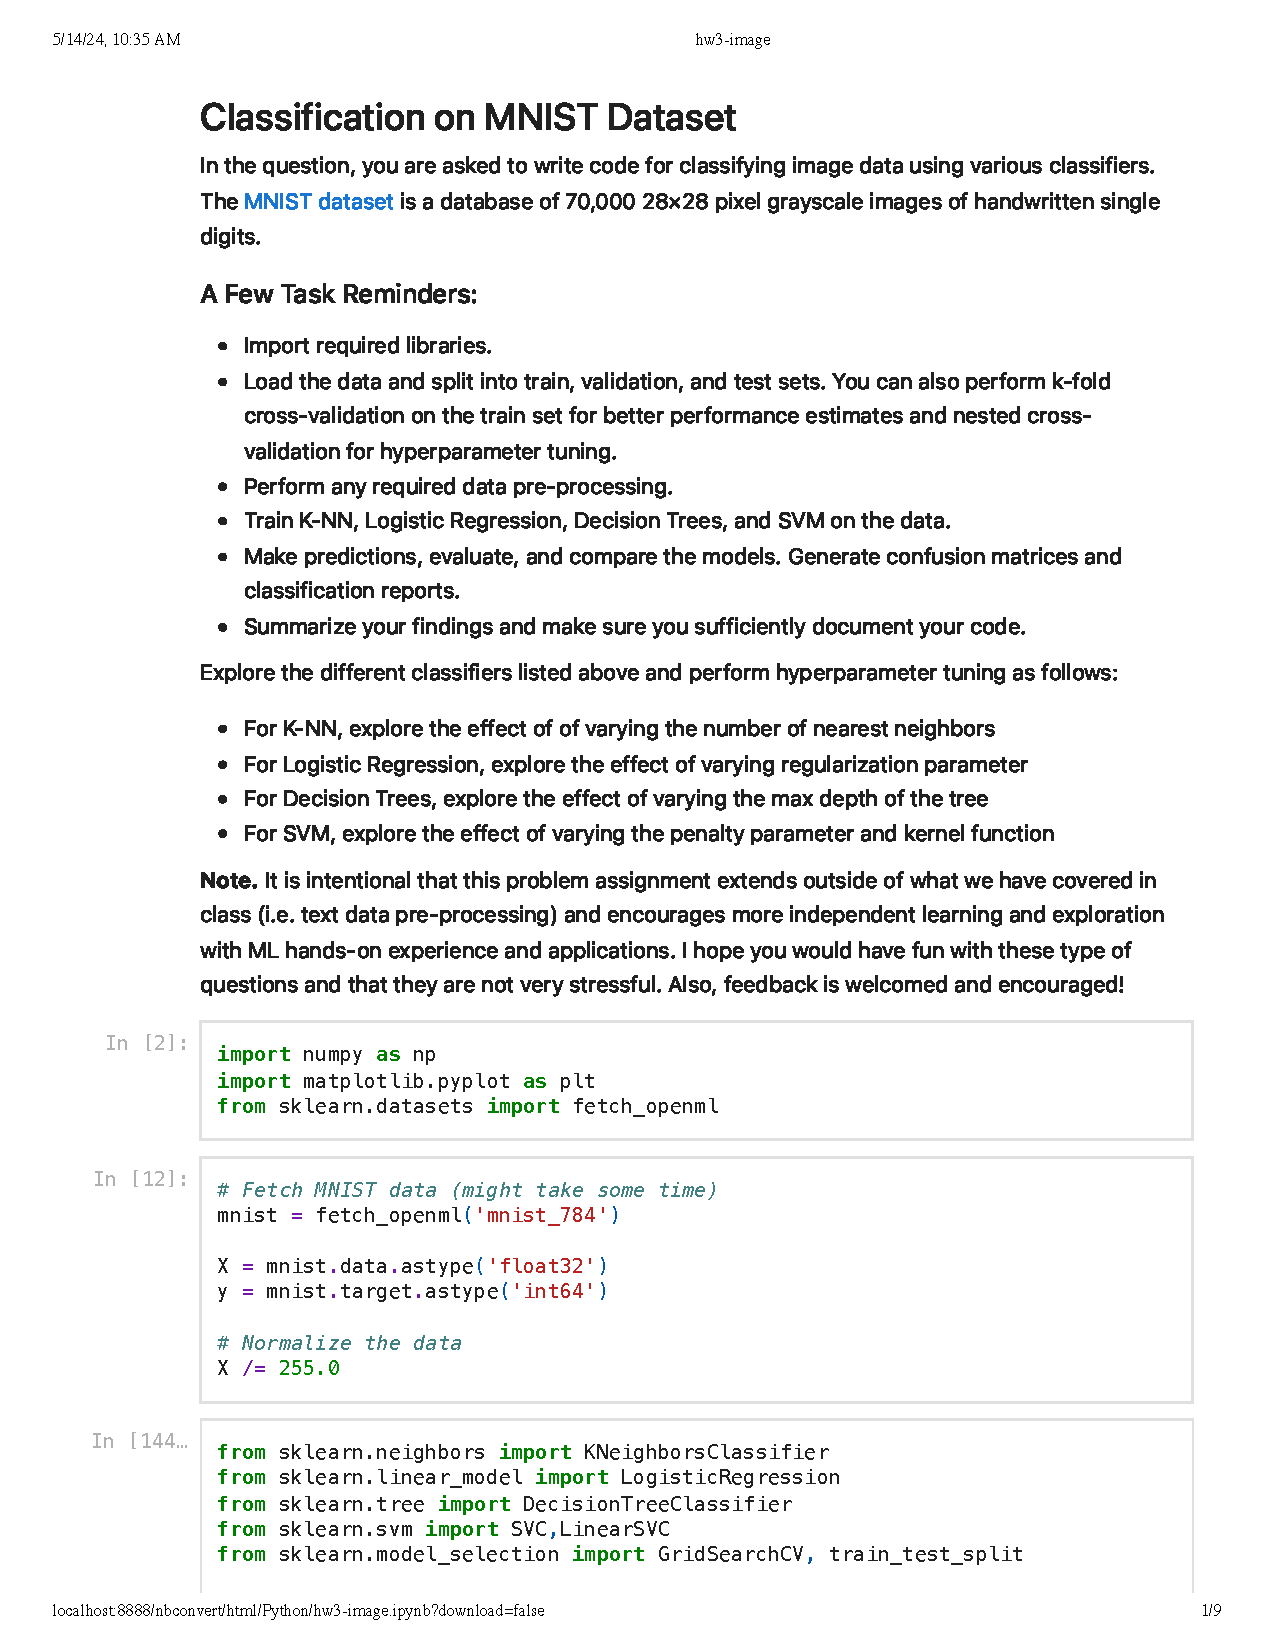
\includepdf[pages=-]{hw3-image.pdf}
\end{document}